\section{Evaluation}
In order to evaluate the usefulness of exploration in \awa, a number of experiments were conducted on the sliding tile puzzle. All experiments are run on an 8-core 1.70GHz machine with 16 gigabytes of memory. For all experiments, the two Exploration Anytime algorithms will be compared to a standard \awa implementation which will serve as the benchmark.

\subsection{Experiment Setup and Overview}
Experiments were conducted on one hundred instances of the unit cost 12-puzzle. The primary focus was on the Unit Cost Sliding Tile puzzle using the Manhattan Distance Heuristic. For this domain, 5 weights are considered for each algorithm, 1.3, 2, 3, 5, and 10. For \eawa and \ebawa, two different values of $\epsilon$ are used, $0.1$ and $0.3$. Depending on the value of $\epsilon$, \eawa and \ebawa will be abbreviated to \e{0.1}, \e{0.3}, \eb{0.1}, and \eb{0.3} respectively. The beta distribution in all \ebawa instances is fixed at $\alpha=5$ and $\beta=0.6$.

There are also two small extensions to the unit cost experiments. In the first, the Inverse Sliding Tile Puzzle is briefly investigated using the Manhattan Distance Heuristic. In these experiments, the value of $\epsilon$ is fixed at 0.3, and only 3 weights are considered: 1.3, 5, and 10. The Inverse Sliding Tile Puzzle was chosen because it tends to be harder than the Unit Cost variant. The second extension involves degrading the heuristic and using the Correct Tile Placement Heuristic. This was done to investigate how exploration may help or hinder with a highly uninformed heuristic.

\subsection{Unit Cost Tile Puzzle}
In general, it was found that adding exploration to AWA* for the sliding tile puzzle proved to be very effective. Both \eawa and \ebawa required fewer incumbent solutions before finding the optimal solution, as summarized in Table \ref{tad:num-sol}.

\begin{table}
\def\arraystretch{1.3}
\begin{tabular}{ |c||c|c|c|c|c|  }
    \hline
    \multicolumn{6}{|c|}{Average Number of Incumbent Solutions} \\
    \hline
    Weight& AWA* & \e{0.1} & \e{0.3} & \eb{0.1} & \eb{0.3}\\
    \hline
    1.3 & \textbf{2.24} & 2.25 & 2.28 & 2.26 & 2.28\\
    \hline
    2 & 3.91 & 4.09 & \textbf{3.75} & 3.94 & 3.86\\
    \hline
    3 & 7.07 & 6.69 & \textbf{6.07} & 6.54 & 6.19\\
    \hline
    5 & 11.15 & 10.37 & \textbf{9.28} & 10.05 & 9.65\\
    \hline
    10& 15.49 & 15.03 & \textbf{13.27} & 14.56 & 13.74\\
    \hline
\end{tabular}
\caption{Unit Cost: Incumbent Solutions}\label{tad:num-sol}
\end{table}

In all cases, except for weight=1.3, $0.1$-\eawa required the fewest incumbent solutions before finding the optimal. However, both exploration techniques were consistently better than standard \awa by this metric. 

To gauge the complexity of each algorithm, the number of expanded nodes and the total number of generated nodes are considered. By this metric exploration shows a huge improvement over standard \awa, as shown in Figure \ref{fig:nodes}.

% \begin{figure*}
%     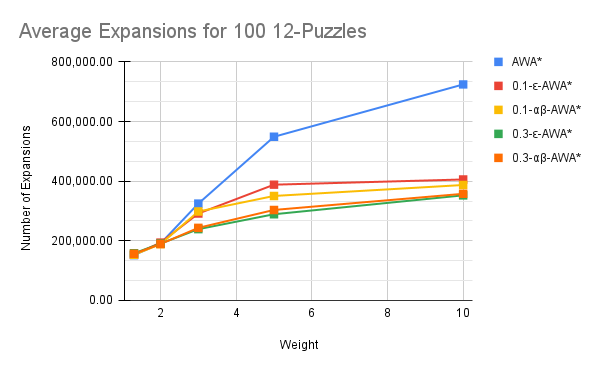
\includegraphics[width=0.47\textwidth]{media/Average Expansions for 100 12-Puzzles.png}
%     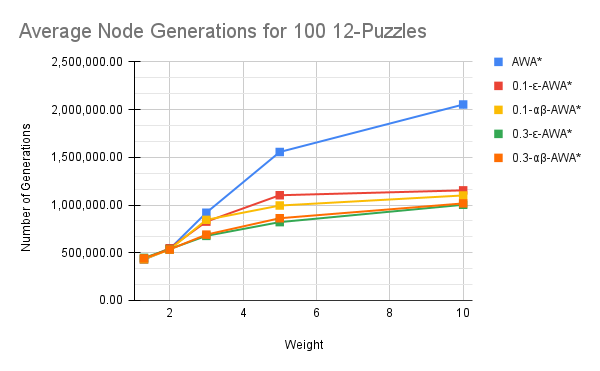
\includegraphics[width=0.47\textwidth]{media/Average Node Generations for 100 12-Puzzles.png}
%     \caption{Complexity with Manhattan Distance Heuristic.} \label{fig:nodes}
% \end{figure*}

\begin{figure}
    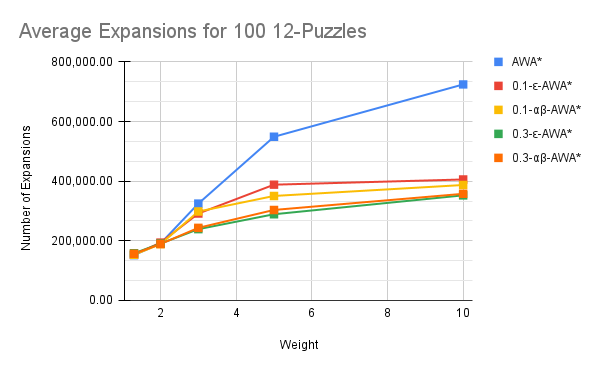
\includegraphics[width=\linewidth]{media/Average Expansions for 100 12-Puzzles.png}
    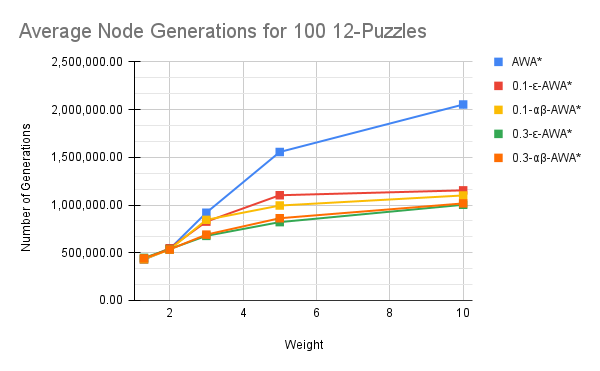
\includegraphics[width=\linewidth]{media/Average Node Generations for 100 12-Puzzles.png}
    \caption{Unit Cost: Complexity} \label{fig:nodes}
\end{figure}

Standard \awa requires close to 800,000 expansions in the case of a weight of 10, while all four exploration algorithms require in the neighbourhood of 400,000. AWA* seems to be far more impacted by increasing the weight, and thereby degrading the accuracy of the evaluation function, than the $\epsilon$ and $\epsilon B$ variants--which both require a similar number of expansions for a weight of 5 and a weight of 10. Perhaps most surprising is that setting $\epsilon$ to 0.3 gets the best results.

Adding to this, exploration in anytime sees an analogous improvement in its runtime when compared to standard \awa, as seen in Figure \ref{fig:run}. This is not guaranteed as it could be the case that the improved node selection procedure takes enough time so as to offset the time savings of expanding fewer nodes. In the cases of \eawa and \ebawa, the node selection procedure is sufficiently simple that the expansion savings result in analogous time savings. 

\begin{figure}
    \begin{center}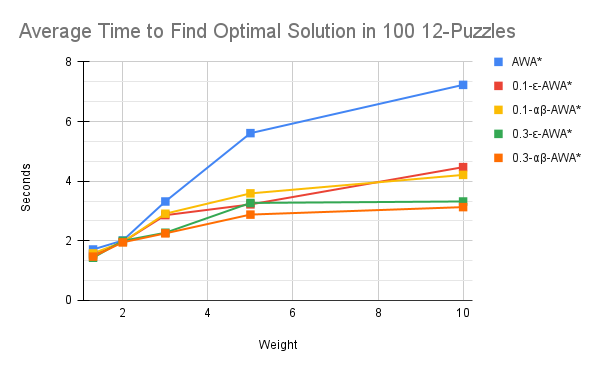
\includegraphics[scale=0.35]{media/Average Time to Find Optimal Solution in 100 12-Puzzles.png}\end{center}
    \caption{Unit Cost: Runtime}\label{fig:run}
\end{figure}

To summarize the above results, it's useful to look at how quickly each algorithm converges on the optimal solution when plotted against time and number of expansions. Given both the $\epsilon$ and $\epsilon B$ variants required fewer incumbent solutions, fewer expansions to get those solutions, and took less time, it should be the case that they approach the optimal solution much faster than \awa, which is precisely what is seen in Figure \ref{fig:conv-man}.


\begin{figure*}
    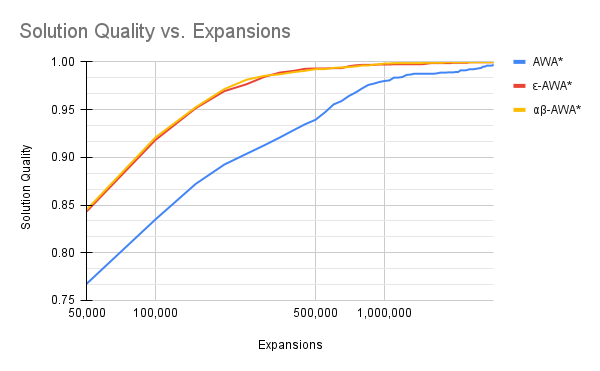
\includegraphics[width=0.47\textwidth]{media/man-Solution Quality vs. Expansions.png}
    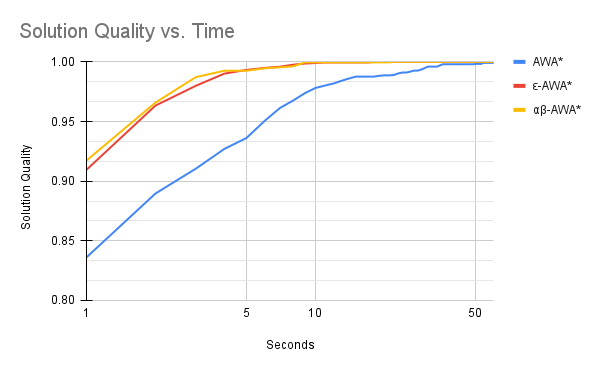
\includegraphics[width=0.47\textwidth]{media/man-Solution Quality vs. Time.png}
    \caption{Unit Cost: Convergence} \label{fig:conv-man}
\end{figure*}

% \begin{figure}
%     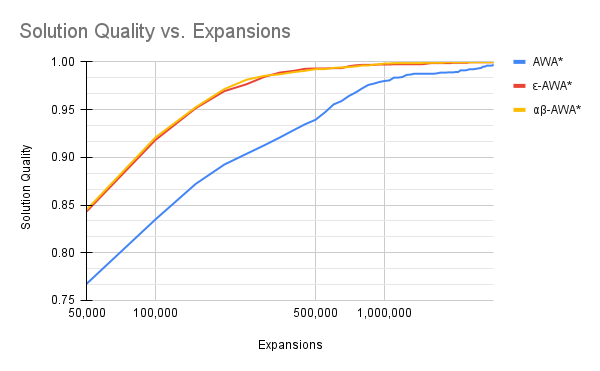
\includegraphics[width=\linewidth]{media/man-Solution Quality vs. Expansions.png}
%     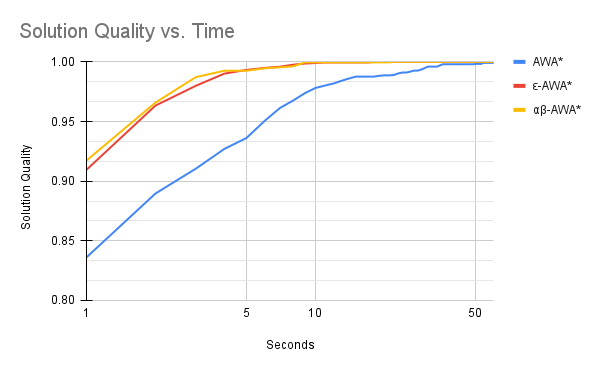
\includegraphics[width=\linewidth]{media/man-Solution Quality vs. Time.png}
%     \caption{Quality Convergence with Manhattan Distance Heuristic.} \label{fig:conv-man}
% \end{figure}

Here, solution quality is $\frac{incumbent-cost}{optimal-cost}$ for a given problem and the solution qualities are averaged across all problem instances. For expansion convergence, the incumbent cost was polled every 50,000 expansions; for the time convergence the incumbent cost was polled every one second (notice the log x-axis in both charts). In this, only a weight of 10 and an epsilon value of 0.3 were considered. 

\subsection{Inverse Cost Tile Puzzle}
Experimenting with the Inverse Cost Tile Puzzle involved the same set of 12-puzzle instances. For these experiments, only weights of 1.3, 5, and 10 were considered and $\epsilon$ was fixed at 0.3 because the  $\epsilon=0.3$ variants performed best in the unit cost problems. 

Exploration also proved very beneficial in the Inverse Tile Puzzle. Table \ref{tab:inv-sol} shows the average number of incumbent solutions found before the optimal is found, and much like the unit cost case, \eawa and \ebawa performed better in all cases and the discrepancy grew with the weight. 

\begin{table}
\def\arraystretch{1.3}
\begin{tabular}{ |c||c|c|c|  }
    \hline
    \multicolumn{4}{|c|}{Average Number of Incumbent Solutions} \\
    \hline
    Weight& AWA* & $0.3$-$\epsilon$-AWA$^*$ & $0.3$-$\epsilon B$-AWA$^*$\\
    \hline
    1.3 & 3.14 & 3.13 & \textbf{2.97} \\
    \hline
    5 & 21.91 & 15.66 & \textbf{15.41} \\
    \hline
    10& 30.8 & \textbf{20.4} & 21.26 \\
    \hline
\end{tabular}
\caption{Inverse Cost: Incumbent Solutions}\label{tab:inv-sol}
\end{table}

The complexity, again taken to be the number of expansions and number of generated nodes, painted a very similar picture to the unit cost case--with the caveat that each algorithm needed twice or more the number of expansions and generations that it did in the unit cost case. As shown in Table \ref{tab:inv-avg-exp}, as the weight increased, \eawa and \ebawa required less than half the number of expansions than \awa did. The difference is even more dramatic than the unit cost case, which was very surprising.

\begin{table}
\def\arraystretch{1.3}
\begin{tabular}{ |c||c|c|c|  }
    \hline
    \multicolumn{4}{|c|}{Average Number of Expansions} \\
    \hline
    Weight& AWA* & $0.3$-$\epsilon$-AWA$^*$ & $0.3$-$\epsilon B$-AWA$^*$\\
    \hline
    1.3 & \textbf{186,038.15} & 211,198.92 & 206,175.07 \\
    \hline
    5 & 1,408,646.74 & 622,837.79 & \textbf{587,692.64} \\
    \hline
    10& 1,901,236.58 & \textbf{709,049.28} & 769,546.95 \\
    \hline
\end{tabular}
\caption{Inverse Cost: Expansions}\label{tab:inv-avg-exp}
\end{table}

Similarly, for the number of generations, while the three algorithms were competitive with a low weight, as the weight increases, the performance of \awa suffers far more dramatically than \eawa and \ebawa. 

\begin{table}
\def\arraystretch{1.3}
\begin{tabular}{ |c||c|c|c|  }
    \hline
    \multicolumn{4}{|c|}{Average Number of Node Generations} \\
    \hline
    Weight& AWA* & $0.3$-$\epsilon$-AWA$^*$ & $0.3$-$\epsilon B$-AWA$^*$\\
    \hline
    1.3 & \textbf{529,095.35} & 603,706.60 & 589,437.60 \\
    \hline
    5 & 4,003,219.50 & 1,780,788.61 & \textbf{1,680,521.61} \\
    \hline
    10& 5,401,559.63 & \textbf{2,027,138.81} & 2,200,575.94 \\
    \hline
\end{tabular}
\caption{Inverse Costs: Generations}\label{tab:inv-avg-gen}
\end{table}

The runtime of the algorithms, unsurprisingly since the domain doesn't affect the time complexity of the sampling, also improved roughly proportionally to the number of required expansions. I believe this is for much the same reason as the unit cost case where since the exploration technique didn't result in much additional work, each saved expansion corresponds to an equivalent time saving. 

\begin{table}
\def\arraystretch{1.3}
\begin{tabular}{ |c||c|c|c|  }
    \hline
    \multicolumn{4}{|c|}{Average Number of Seconds to Find Optimal} \\
    \hline
    Weight& AWA* & $0.3$-$\epsilon$-AWA$^*$ & $0.3$-$\epsilon B$-AWA$^*$\\
    \hline
    1.3 & 2.25 & \textbf{2.15} & \textbf{2.15} \\
    \hline
    5 & 16.38 & 6.65 & \textbf{6.34} \\
    \hline
    10& 21.57 & \textbf{7.3} & 8.09 \\
    \hline
\end{tabular}
\caption{Inverse Costs: Runtime}\label{tab:inv-avg-time}
\end{table}

All in all, I was very surprised and impressed with the efficacy of both exploration techniques in the Inverse Tile Problem. Because it is a harder problem with I believe fewer plateaus, I expected more modest results. 

\subsection{Degraded Heuristic in Unit Cost Sliding Tiles}
Given the promising results above, it would be expected that when the heuristic gets degraded exploration should help even more, as degraded heuristics result in more plateaus and less confidence about the `best' node in the open list. However, in looking at the summary evaluation of solution quality over time and expansions using the Correct Tile Placement Heuristic, this did not turn out to be case, as seen in Figure \ref{fig:conv-correct}.

Here, again, only a weight of 10 and an epsilon value of 0.3 were considered. For expansions, each algorithm was limited to 3,000,000, and for runtime each algorithm was limited to one minute. 

\begin{figure*}
    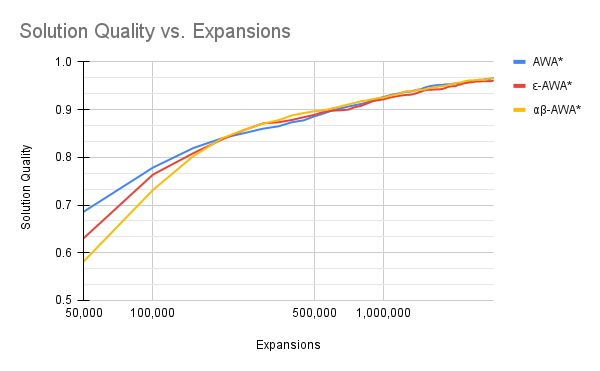
\includegraphics[width=0.47\textwidth]{media/correct-Solution Quality vs. Expansions.png}
    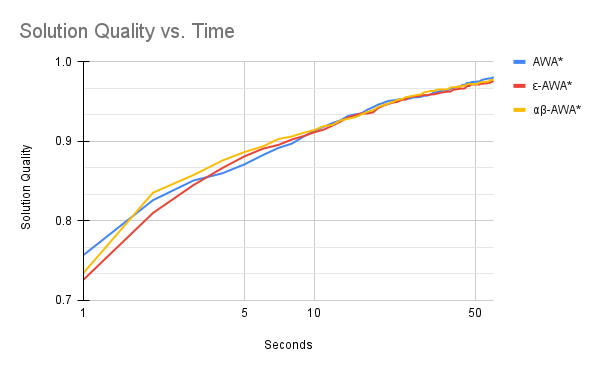
\includegraphics[width=0.47\textwidth]{media/correct-Solution Quality vs. Time.png}
    \caption{Unit Cost: Convergence with Degrade Heuristic} \label{fig:conv-correct}
\end{figure*}

% \begin{figure}
%     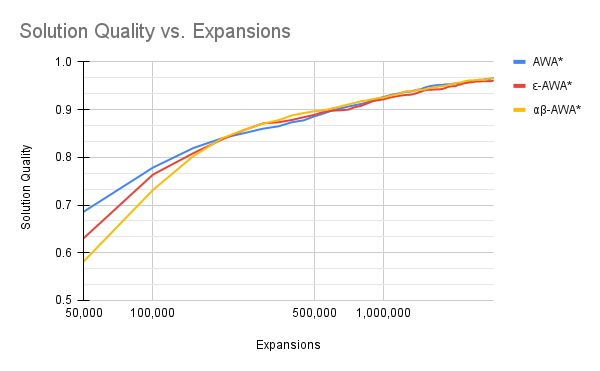
\includegraphics[width=\linewidth]{media/correct-Solution Quality vs. Expansions.png}
%     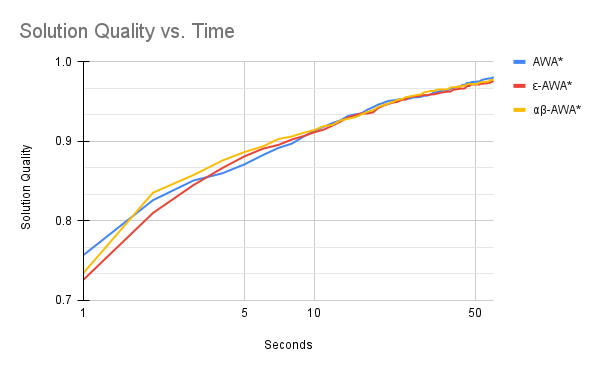
\includegraphics[width=\linewidth]{media/correct-Solution Quality vs. Time.png}
%     \caption{Quality Convergence with Correct Tile Placement Heuristic.} \label{fig:conv-correct}
% \end{figure}

While in the beginning \awa actually acquires the best incumbent solutions, they all more or less approach the optimal solution at the same rate. This seems to simply demonstrate just how bad the Correct Placement Heuristic is. I think what is going on here is that the Correct Placement Heuristic is so bad it affectively adds and pulls nodes from the open list at random and so adding an exploration technique in no way helps since choosing the `best' node is also, in effect, exploratory.

% \begin{figure*}
% 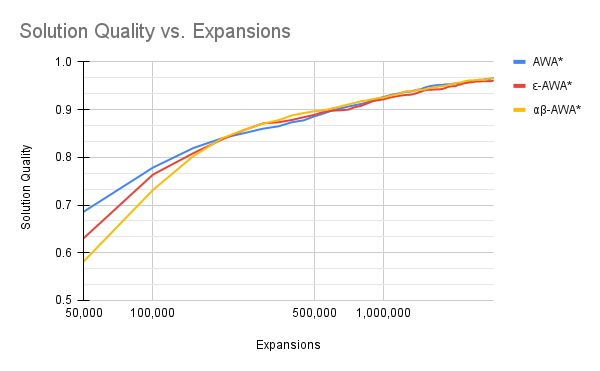
\includegraphics{media/correct-Solution Quality vs. Expansions.png}
% 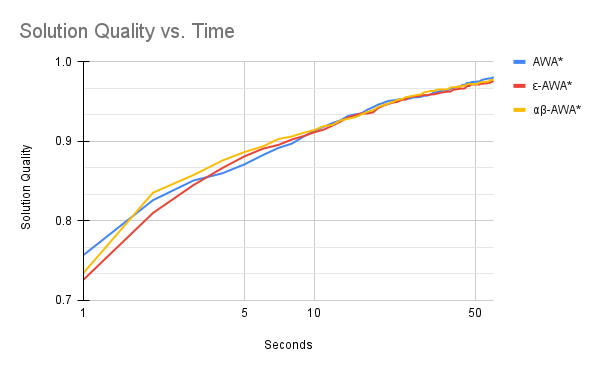
\includegraphics{media/correct-Solution Quality vs. Time.png}
% \caption{Quality Convergence with a Bad Heuristic.} \label{fig:conv-correct}
% \end{figure*}

